\documentclass[aspectratio=169,11pt]{beamer}
% 6-minute talk: 8 slides (title + 7), ~45 s each. Backup slides come after \appendix.

%===============================================================================
%  PACKAGES
%===============================================================================
\usepackage[utf8]{inputenc}
\usepackage[T1]{fontenc}
\usepackage{lmodern}
\usepackage{amsmath, amssymb, bm}
\usepackage{booktabs}
\usepackage{graphicx}
\usepackage{tikz}
\usetikzlibrary{arrows.meta, positioning, shapes.geometric}
\usepackage[authoryear,round]{natbib}

%===============================================================================
%  THEME (lightweight custom theme on top of the default one)
%===============================================================================
\usetheme{default}
\definecolor{mvablue}{RGB}{20,60,110}
\definecolor{mvaaccent}{RGB}{215,110,30}
\definecolor{mvagray}{RGB}{110,110,110}

\setbeamercolor{structure}{fg=mvablue}
\setbeamercolor{frametitle}{fg=white,bg=mvablue}
\setbeamercolor{title}{fg=mvablue}
\setbeamercolor{alerted text}{fg=mvaaccent}
\setbeamercolor{block title}{fg=white,bg=mvablue}
\setbeamercolor{block body}{bg=mvablue!6}
\setbeamerfont{frametitle}{series=\bfseries}
\setbeamerfont{title}{series=\bfseries,size=\LARGE}
\setbeamertemplate{navigation symbols}{}
\setbeamertemplate{itemize items}[circle]
\setbeamertemplate{blocks}[rounded][shadow=false]
\setbeamertemplate{bibliography item}{}

\setbeamertemplate{frametitle}{%
  \nointerlineskip
  \begin{beamercolorbox}[wd=\paperwidth,ht=2.4ex,dp=1.2ex,leftskip=1em]{frametitle}
    \usebeamerfont{frametitle}\insertframetitle
  \end{beamercolorbox}%
}

% Footer: "n / 8" in the main talk, "Backup" in the appendix.
\newif\ifbackup
\newcommand{\mainslides}{8}
\setbeamertemplate{footline}{%
  \leavevmode\hbox{%
    \begin{beamercolorbox}[wd=\paperwidth,ht=2.5ex,dp=1ex,leftskip=1em,rightskip=1em]{}
      \color{mvagray}\scriptsize
      \insertshortauthor\ \textbar\ \insertshorttitle\hfill
      \ifbackup Backup\else\insertframenumber\,/\,\mainslides\fi
    \end{beamercolorbox}}%
}

%===============================================================================
%  HELPERS
%===============================================================================
% Highlight a number/claim that still has to be checked against the paper.
% Turn it off for the final version with: \renewcommand{\verify}[1]{#1}
\newcommand{\verify}[1]{\colorbox{yellow!50}{#1}}
% Speaker TODO, rendered in red. Remove before presenting.
\newcommand{\todo}[1]{{\color{red}\footnotesize[TODO: #1]}}
% Include a figure if it exists in figures/, otherwise draw a placeholder box.
\newcommand{\figorplaceholder}[2]{%
  \IfFileExists{figures/#1}{\includegraphics[#2]{figures/#1}}{%
    \fbox{\parbox[c][0.4\textheight][c]{0.9\linewidth}{\centering\color{mvagray}\footnotesize\ttfamily figures/\detokenize{#1}}}}%
}

\newcommand{\X}{\mathbf{X}}

%===============================================================================
%  TITLE
%===============================================================================
\title[GenCast]{GenCast: Probabilistic Weather Forecasting\\with Machine Learning}
\subtitle{Paper presentation \textbar\ \citet{price2025gencast}, \emph{Nature}}
\author[N.\ Ugwonali]{Nathan Ugwonali}
\institute{MVA \textbar\ ALTEGRAD: Advanced Learning for Text and Graph Data}
\date{3 December 2026}

\begin{document}

%===============================================================================
% 1. Title  (~15 s)
%===============================================================================
\begin{frame}[plain]
  \titlepage
\end{frame}

%===============================================================================
% 2. Motivation  (~50 s)
%===============================================================================
\begin{frame}{Why this paper?}
  \begin{itemize}
    \item The atmosphere is \alert{chaotic}: a single forecast is not enough, we need a \emph{distribution} over futures.
    \item Today: physics-based \alert{ensembles} (ECMWF ENS, \verify{50 members}), very expensive to run.
    \item ML forecasters (GraphCast) beat physics, but are \emph{deterministic}: trained with MSE, they blur and give no uncertainty.
  \end{itemize}
  \vfill
  \begin{block}{Why I chose it}
    It sits exactly where I want to do research, \alert{ML for applied physics}: a generative model that learns a chaotic physical system,
    respects its geometry, and is judged against the best physics-based baseline.
    \todo{rephrase in your own words}
  \end{block}
\end{frame}

%===============================================================================
% 3. Task  (~45 s)
%===============================================================================
\begin{frame}{Task: sampling weather trajectories}
  \begin{itemize}
    \item State $\X^t$: \verify{6 surface + 6 atmospheric variables $\times$ 13 levels} on a \verify{$0.25^\circ$} global grid.
    \item Goal: sample 15-day trajectories, with a Markov factorisation over \verify{12\,h} steps:
      \[
        p(\X^{1:T}\mid \X^{0},\X^{-1}) \;=\; \prod_{t=0}^{T-1} p_\theta\big(\X^{t+1} \mid \X^{t}, \X^{t-1}\big).
      \]
    \item \alert{Autoregressive sampling}: each sampled state is fed back as input $\Rightarrow$ one coherent trajectory per member.
    \item Ensemble = $N$ independent trajectories, started from \verify{ERA5 + ensemble-analysis perturbations}.
  \end{itemize}
\end{frame}

%===============================================================================
% 4. Diffusion  (~50 s)
%===============================================================================
\begin{frame}{Each step is a conditional diffusion model}
  \begin{itemize}
    \item Generate the \alert{residual} $\mathbf{Z} = \X^{t+1} - \X^{t}$ \verify{(normalised)}, conditioned on $(\X^{t}, \X^{t-1})$.
    \item Denoiser trained on all noise levels $\sigma$ \citep[EDM-style,][]{karras2022edm}:
      \[
        \mathcal{L}(\theta) = \mathbb{E}\Big[\lambda(\sigma)\,\big\| D_\theta(\mathbf{Z}+\sigma\bm{\varepsilon};\,\X^{t},\X^{t-1},\sigma) - \mathbf{Z}\big\|^2\Big].
      \]
    \item Noise $\bm{\varepsilon}$ sampled in \alert{spherical-harmonic} space: isotropic on the globe, not denser at the poles of the lat--lon grid.
    \item Sampling: \verify{DPM-Solver++ 2S, 20 steps} per 12\,h step.
  \end{itemize}
\end{frame}

%===============================================================================
% 5. Architecture -- the graph part  (~55 s)
%===============================================================================
\begin{frame}{The denoiser: a graph transformer on the sphere}
  \centering
  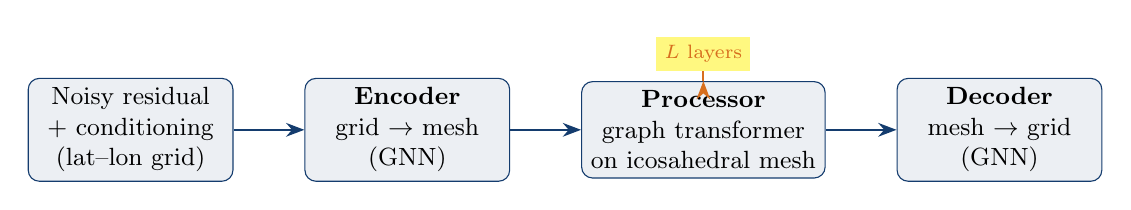
\begin{tikzpicture}[
      node distance=0.9cm,
      box/.style={draw=mvablue, fill=mvablue!8, rounded corners, minimum width=2.6cm, minimum height=1.1cm, align=center, font=\small},
      arr/.style={-{Stealth}, thick, mvablue}]
    \node[box] (in)  {Noisy residual\\+ conditioning\\(lat--lon grid)};
    \node[box, right=of in]  (enc) {\textbf{Encoder}\\grid $\to$ mesh\\(GNN)};
    \node[box, right=of enc] (proc) {\textbf{Processor}\\graph transformer\\on icosahedral mesh};
    \node[box, right=of proc] (dec) {\textbf{Decoder}\\mesh $\to$ grid\\(GNN)};
    \draw[arr] (in) -- (enc);
    \draw[arr] (enc) -- (proc);
    \draw[arr] (proc) -- (dec);
    \draw[arr, mvaaccent] (proc.north) to[out=60,in=120,looseness=4] node[above, font=\scriptsize]{\verify{$L$ layers}} (proc.north);
  \end{tikzpicture}
  \vfill
  \raggedright
  \begin{itemize}
    \item Mesh: icosahedron refined \verify{6 times} (\verify{$\sim$41k nodes}), near-uniform on the sphere.
    \item vs GraphCast: \verify{single mesh} instead of multi-mesh, \alert{attention over $k$-hop neighbourhoods} instead of MLP message passing.
    \item Course link: the mesh's graph-Laplacian eigenvectors \alert{are the spherical harmonics} (checked numerically, backup). Spectral graph theory on the mesh = harmonic analysis on the sphere.
  \end{itemize}
\end{frame}

%===============================================================================
% 6. Results  (~60 s)
%===============================================================================
\begin{frame}{Results against ECMWF ENS}
  \begin{columns}[c]
    \begin{column}{0.5\textwidth}
      \centering
      \figorplaceholder{crps_scorecard.pdf}{width=\linewidth}\\[2pt]
      {\scriptsize CRPS scorecard, GenCast vs ENS \todo{export from paper}}
    \end{column}
    \begin{column}{0.48\textwidth}
      \begin{itemize}
        \item Better \alert{CRPS} on \verify{97.2\%} of \verify{1320} targets (variable $\times$ level $\times$ lead time).
        \item Well \alert{calibrated}: spread/skill $\approx 1$.
        \item Better on \alert{extremes}, \alert{cyclone tracks} and regional \alert{wind power}.
        \item 15-day member in \verify{8 min} on one \verify{TPU v5}.
      \end{itemize}
    \end{column}
  \end{columns}
\end{frame}

%===============================================================================
% 7. Critical assessment  (~50 s)
%===============================================================================
\begin{frame}{Critical assessment}
  \begin{columns}[T]
    \begin{column}{0.48\textwidth}
      \textbf{Strengths}
      \begin{itemize}
        \item Rigorous probabilistic evaluation against the \emph{strongest} operational baseline.
        \item Samples are full trajectories: usable for downstream tasks (cyclones, energy).
        \item Geometry-aware design: mesh on the sphere, isotropic noise.
      \end{itemize}
    \end{column}
    \begin{column}{0.48\textwidth}
      \textbf{Limitations}
      \begin{itemize}
        \item Still needs NWP \alert{data assimilation} for its initial conditions.
        \item Each step is an iterative sampler: \alert{costly} compared with one forward pass.
        \item No explicit physical constraints (e.g.\ conservation laws); generalisation to a \alert{changing climate} unclear.
      \end{itemize}
    \end{column}
  \end{columns}
\end{frame}

%===============================================================================
% 8. Take-aways  (~35 s)
%===============================================================================
\begin{frame}{Take-aways and open questions}
  \begin{block}{Take-aways}
    \begin{itemize}
      \item Generative models + GNNs on the sphere now beat the best physics-based ensemble.
      \item The gain comes from \emph{sampling} the dynamics instead of regressing their mean.
    \end{itemize}
  \end{block}
  \begin{block}{Open questions (ML $\times$ physics)}
    \begin{itemize}
      \item Learn data assimilation too, directly from observations?
      \item Build physical constraints into generative surrogates of chaotic systems?
    \end{itemize}
  \end{block}
  \vfill
  \centering{\color{mvablue}\large\bfseries Thank you! Questions?}
\end{frame}

%===============================================================================
%  BACKUP (not part of the 6-minute talk)
%===============================================================================
\appendix
\backuptrue

\begin{frame}[allowframebreaks]{References}
  \footnotesize
  \bibliographystyle{plainnat}
  \nocite{lam2023graphcast, hersbach2020era5}
  \bibliography{references}
\end{frame}

\begin{frame}{Backup: spherical harmonics and the graph Laplacian}
  \begin{columns}[T]
    \begin{column}{0.48\textwidth}
      \textbf{Sphere}
      \begin{itemize}
        \item $\Delta_{S^2} Y_\ell^m = -\ell(\ell+1)\,Y_\ell^m$
        \item Degree $\ell$ = spatial scale ($\approx 40\,000$\,km$/\ell$)
        \item Used for isotropic diffusion noise and power spectra
      \end{itemize}
    \end{column}
    \begin{column}{0.48\textwidth}
      \textbf{Graph}
      \begin{itemize}
        \item $L u_k = \lambda_k u_k$, \quad $L = D - A$
        \item Small $\lambda_k$ = smooth signals on the graph
        \item Spectral clustering, spectral GNNs (ChebNet, GCN)
      \end{itemize}
    \end{column}
  \end{columns}
  \vfill
  On a fine icosahedral mesh, the low eigenvectors of the mesh Laplacian approximate the low-degree spherical harmonics.
\end{frame}

\begin{frame}{Backup: the icosahedral mesh ``knows'' the spherical harmonics}
  \centering
  \figorplaceholder{laplacian_spectrum.pdf}{width=0.92\textwidth}
  \vfill
  \raggedright\small
  Mesh with 2562 nodes, $L = D - A$. Plateaus of width $2\ell+1$ at $\propto \ell(\ell+1)$ (scale $c \approx \tfrac32 h^2$);
  eigenvectors have $>96\%$ of their energy in $\mathrm{span}\{Y_\ell^m\}$ for $\ell \leq 10$.
  Plateaus split ($\ell=3$: $3+4$, $\ell=5$: $3+3+5$, \dots) following the irreducible representations of the \alert{icosahedral group}.
\end{frame}

\begin{frame}{Backup: why sample diffusion noise in spherical-harmonic space}
  \begin{columns}[c]
    \begin{column}{0.52\textwidth}
      \centering
      \figorplaceholder{noise_isotropy.pdf}{width=\linewidth}
    \end{column}
    \begin{column}{0.45\textwidth}
      \small
      \begin{itemize}
        \item i.i.d.\ noise per lat--lon pixel: lat--lon cells shrink near the poles, so large-scale noise power drops to \alert{$0.19\times$} at $80^\circ$.
        \item White noise in spherical-harmonic space ($\hat\varepsilon_{\ell m} \sim \mathcal N(0,1)$): \alert{flat}, i.e.\ isotropic.
        \item Isotropic Gaussian field $\Leftrightarrow$ independent $\hat\varepsilon_{\ell m}$ with variance depending only on $\ell$.
      \end{itemize}
    \end{column}
  \end{columns}
\end{frame}

\begin{frame}{Backup: GraphCast vs GenCast}
  \centering
  \begin{tabular}{lll}
    \toprule
                 & \textbf{GraphCast} \citep{lam2023graphcast} & \textbf{GenCast} \\
    \midrule
    Output       & deterministic state & sample from a distribution \\
    Mesh         & multi-mesh (all refinements) & \verify{single refined mesh} \\
    Processor    & message passing (MLPs on edges) & \verify{graph transformer} \\
    Training     & MSE + autoregressive fine-tuning & denoising (diffusion) \\
    Uncertainty  & none & ensemble of trajectories \\
    \bottomrule
  \end{tabular}
\end{frame}

\end{document}
